\documentclass[12pt,fleqn]{article}\usepackage{../../common}
\begin{document}
M��teri Sadakatini Tahmin Etmek (Churn Prediction)


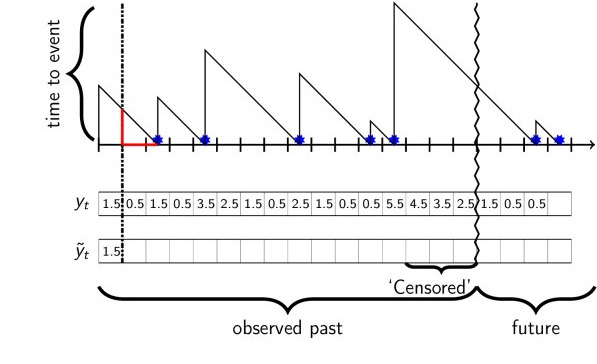
\includegraphics[width=20em]{censor-0.jpg}
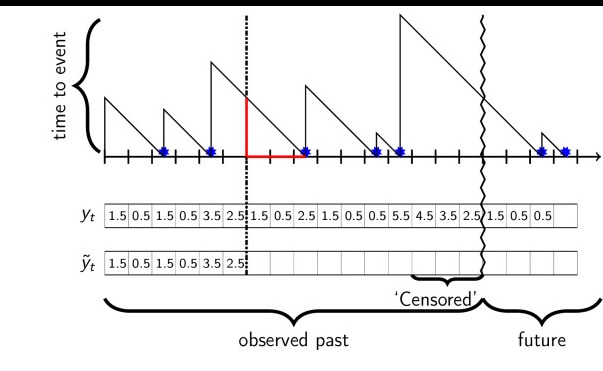
\includegraphics[width=21em]{censor-5.jpg}

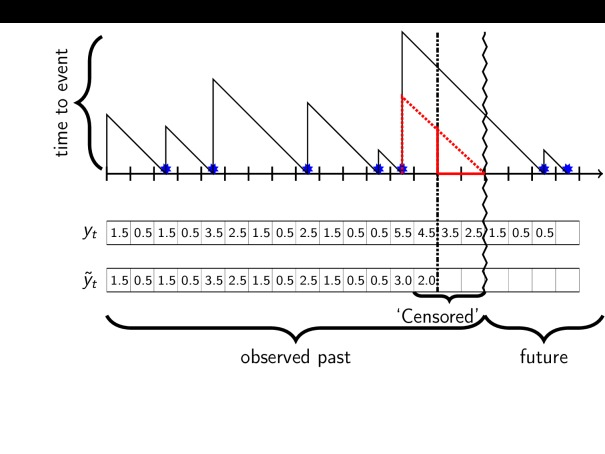
\includegraphics[width=20em]{censor-13.jpg}
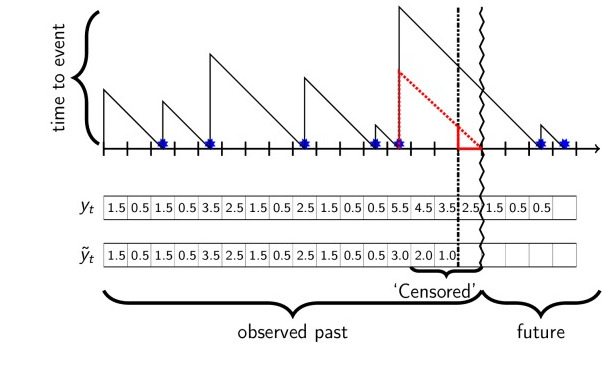
\includegraphics[width=20em]{censor-14.jpg}

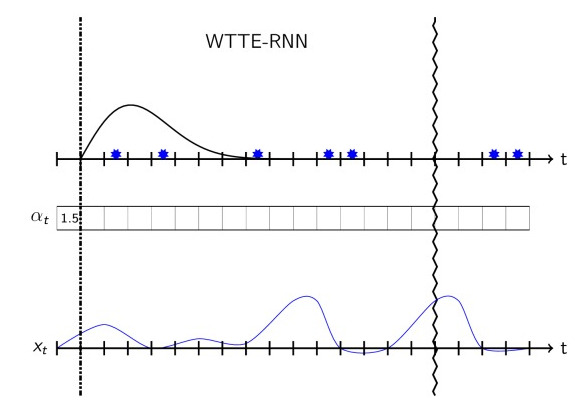
\includegraphics[width=20em]{wtte-0.jpg}
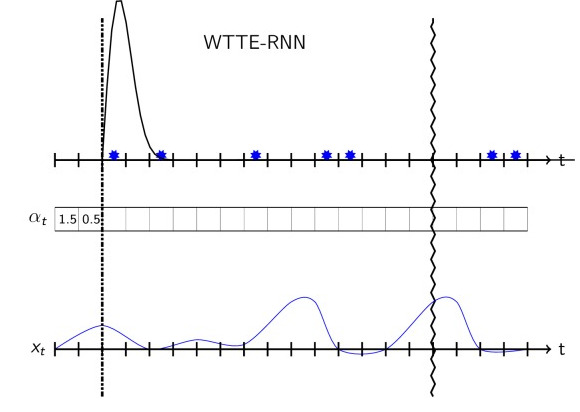
\includegraphics[width=20em]{wtte-1.jpg}

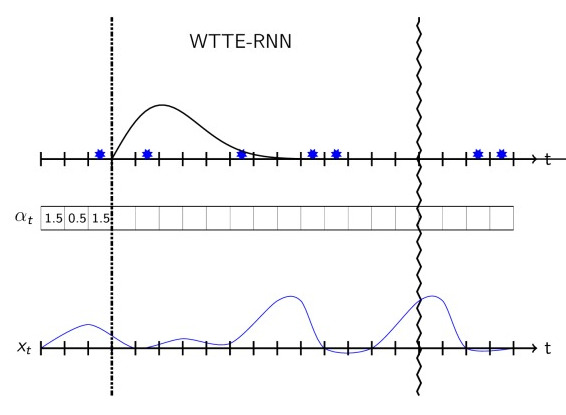
\includegraphics[width=20em]{wtte-2.jpg}
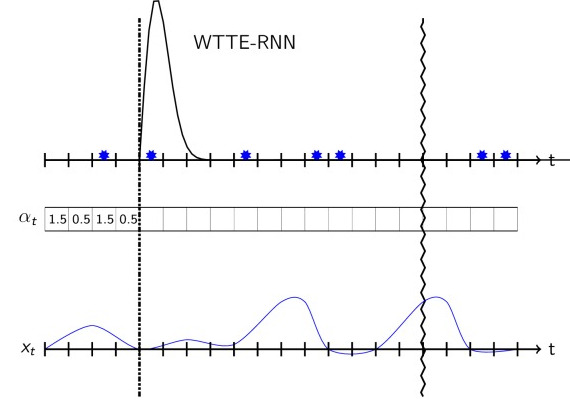
\includegraphics[width=20em]{wtte-3.jpg}

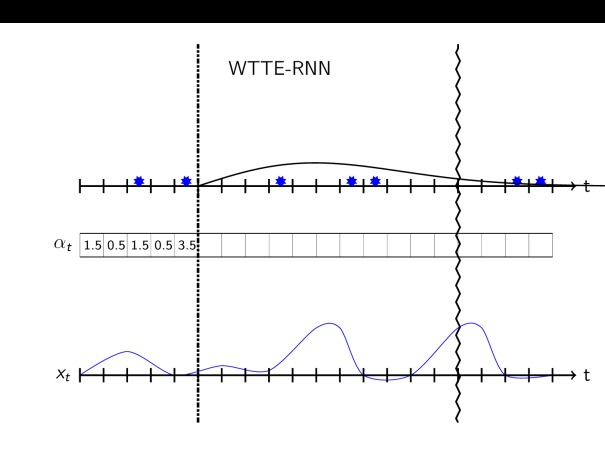
\includegraphics[width=20em]{wtte-4.jpg}
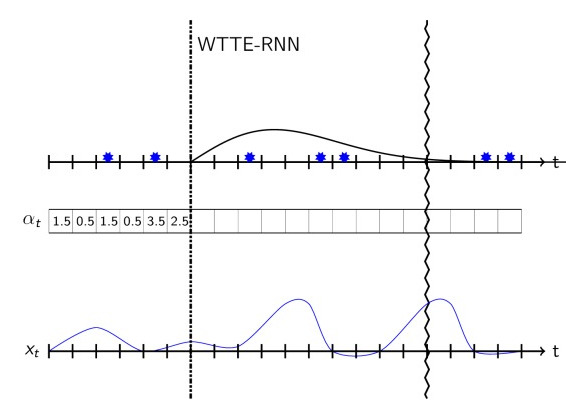
\includegraphics[width=20em]{wtte-5.jpg}

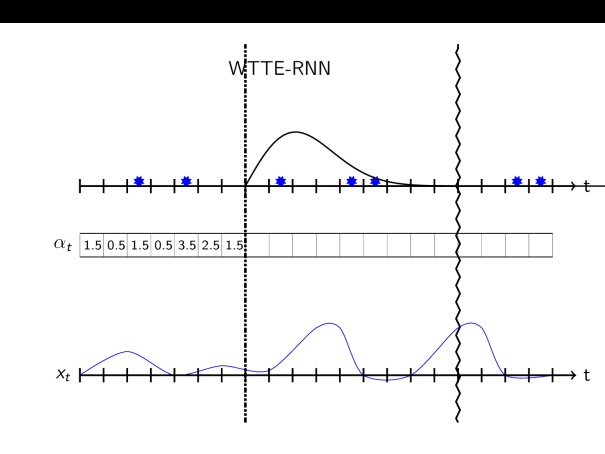
\includegraphics[width=20em]{wtte-6.jpg}
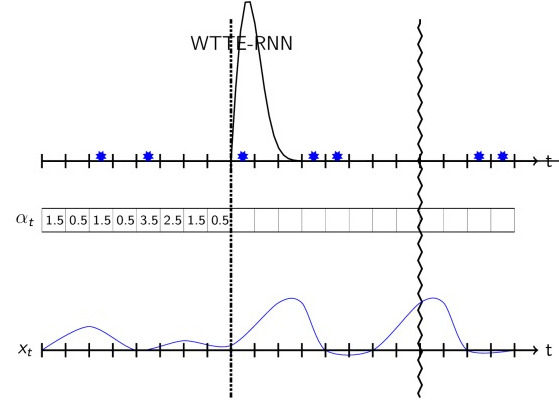
\includegraphics[width=20em]{wtte-7.jpg}

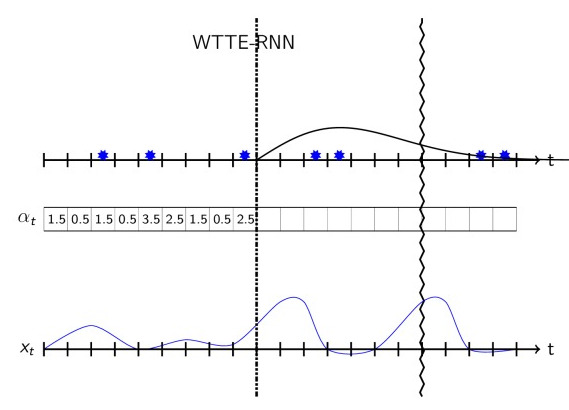
\includegraphics[width=20em]{wtte-8.jpg}
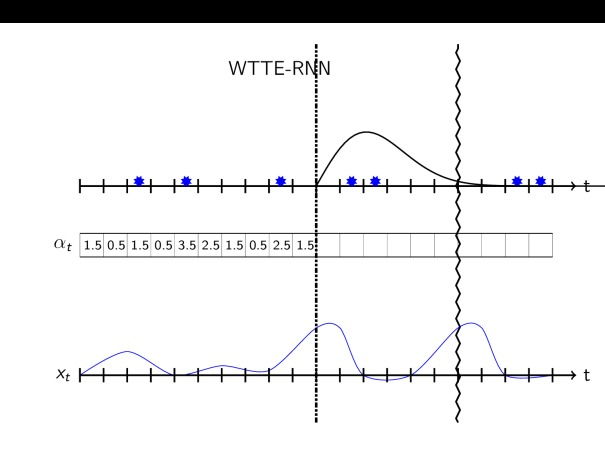
\includegraphics[width=20em]{wtte-9.jpg}

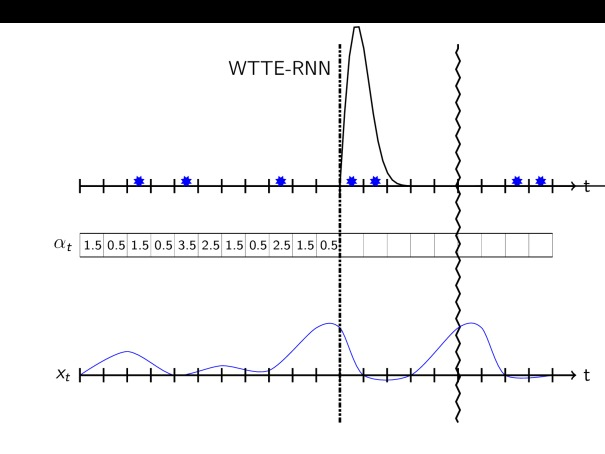
\includegraphics[width=20em]{wtte-10.jpg}
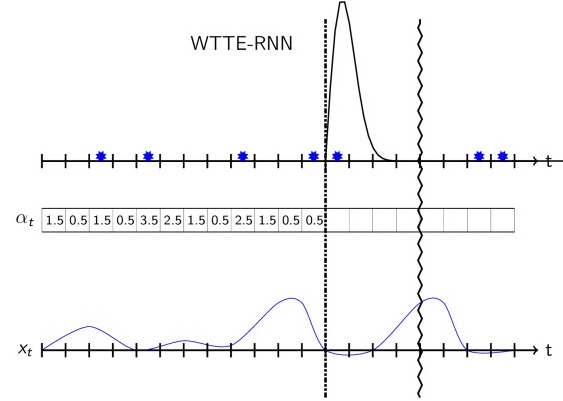
\includegraphics[width=20em]{wtte-11.jpg}







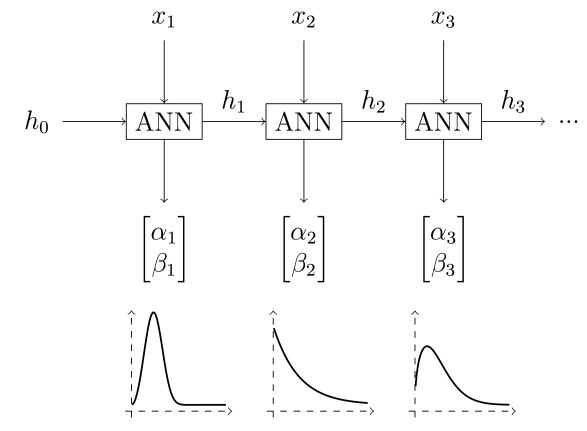
\includegraphics[width=30em]{wtte-rnn.png}




Kaynaklar

[1] Egil, {\em WTTE-RNN - Less hacky churn prediction}, \url{https://ragulpr.github.io/2016/12/22/WTTE-RNN-Hackless-churn-modeling/}

[2] Egil, {\em WTTE-RNN : Weibull Time To Event Recurrent Neural Network}, \url{https://ragulpr.github.io/assets/draft_master_thesis_martinsson_egil_wtte_rnn_2016.pdf}

[3] Bayramli, Parakende Veri Dosyasi, \url{https://www.dropbox.com/s/anlijprxktjqx3x/retail.zip?dl=1}

[4] GraphLab, {\em Churn Prediction}, \url{https://turi.com/learn/userguide/churn_prediction/quick-start.html}

\end{document}
